\documentclass{beamer}
\usepackage{color,amsmath}
\usepackage{subfigure}
\usepackage{booktabs}
\usepackage{framed}
\usepackage{comment}

\def\vf{\vfill}

%%%%%%%%%%%%%%%%%%%%%%%%%%
\title[]{Four areas of difficulty:\\Informed consent, informational risk, privacy, and making decisions in the face of uncertainty}
\author[]{Matthew J. Salganik\\Department of Sociology\\Princeton University}
\date[]{Summer Institute in Computational Social Science\\June 19, 2017
\vfill
\begin{flushright}
\vspace{0.6in}

\includegraphics[width=0.1\textwidth]{figures/cc-by.png}
\end{flushright}
}
\begin{document}
%%%%%%%%%%%%%%%%%%%%%%%%%%
\frame{\titlepage}
%%%%%%%%%%%%%%%%%%%%%%%%%%
\begin{frame}

Informed consent

\end{frame}
%%%%%%%%%%%%%%%%%%%%%%%%%%%
\begin{frame}

Understanding and managing informational risk

\end{frame}
%%%%%%%%%%%%%%%%%%%%%%%%%%%
\begin{frame}

\begin{center}
\only<1>{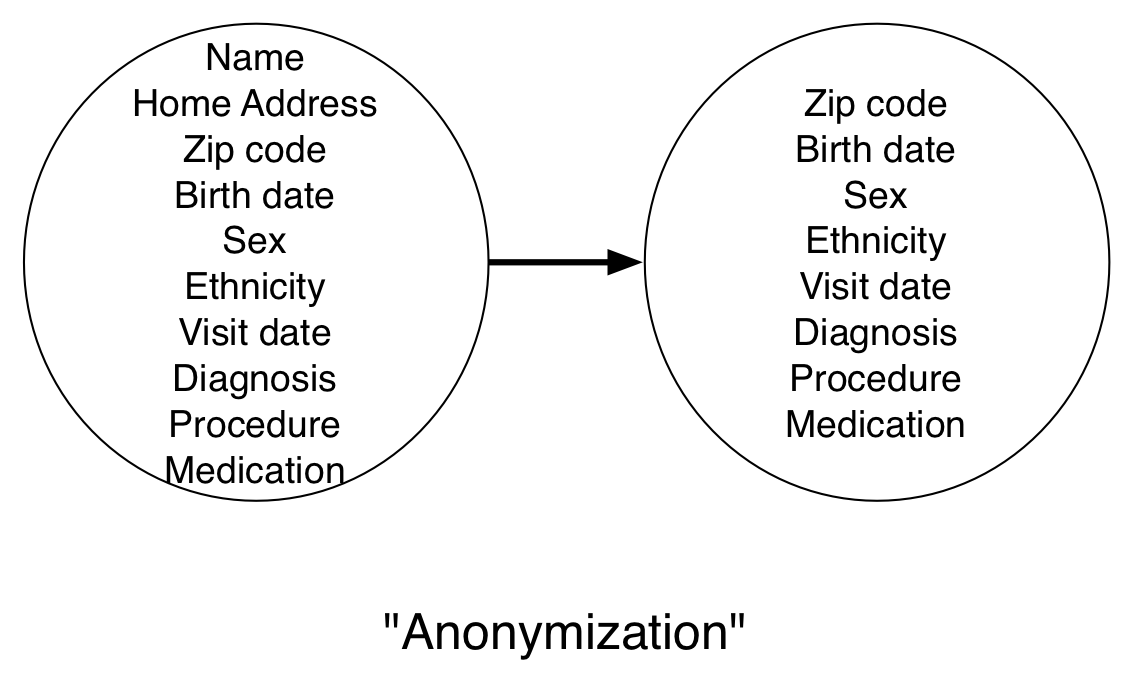
\includegraphics[width=0.9\textwidth]{figures/anonymization.png}}
\only<2>{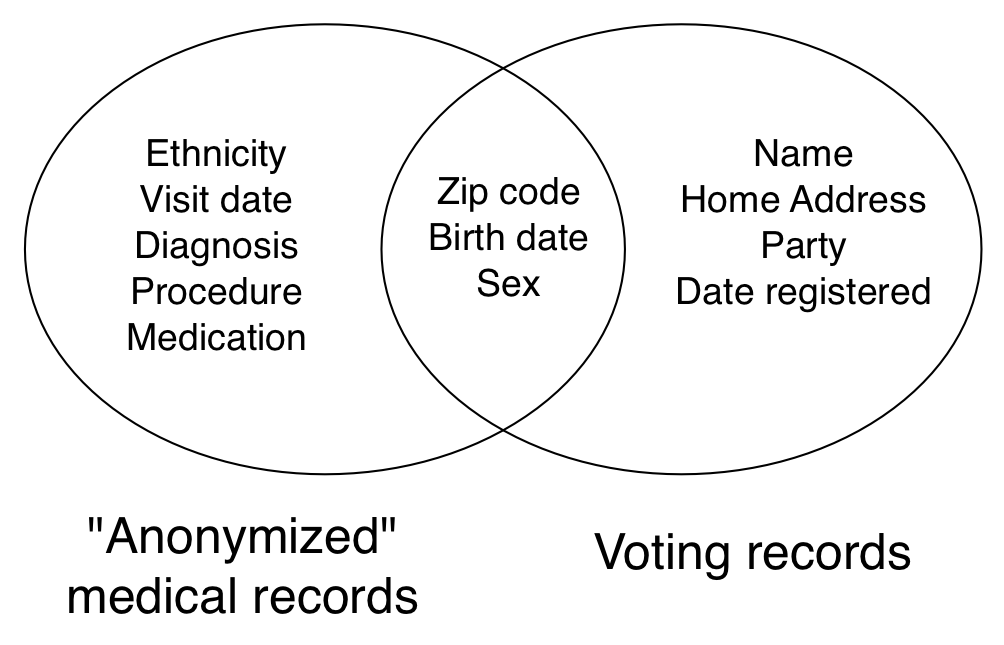
\includegraphics[width=0.9\textwidth]{figures/re-identified.png}}
\end{center}

\end{frame}
%%%%%%%%%%%%%%%%%%%%%%%%%%%
\begin{frame}

Risks come from combining data sources\\
\vf
\begin{minipage}[c]{0.35\textwidth}
$\underbrace{\text{Baking soda}}_{\text{Safe}} + \underbrace{\text{Vinegar}}_{\text{Safe}} =$
\end{minipage}
\hspace{0.05\textwidth}
\begin{minipage}[c]{0.55\textwidth}
\onslide<2>{
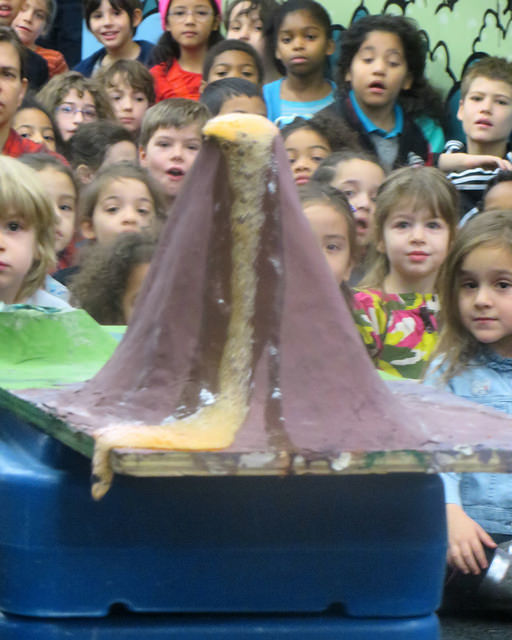
\includegraphics[width=0.8\textwidth]{figures/baking_soda_volcano}\\ {\tiny \url{https://www.flickr.com/photos/edenpictures/15962352215/}}
}
\end{minipage}

\end{frame}
%%%%%%%%%%%%%%%%%%%%%%%%%%
\begin{frame}

Privacy

\end{frame}
%%%%%%%%%%%%%%%%%%%%%%%%%%%
\begin{frame}

What is privacy?

\end{frame}
%%%%%%%%%%%%%%%%%%%%%%%%%%%
\begin{frame}

Making decisions in the face of uncertainty

\end{frame}
%%%%%%%%%%%%%%%%%%%%%%%%%%%
\begin{frame}

\begin{itemize}
\item IRB is a floor not a ceiling
\pause
\item Put yourself in everyone else's shoes
\pause
\item Think of research ethics as continuous not discrete
\end{itemize}

\end{frame}

%%%%%%%%%%%%%%%%%%%%%%%%%%
%%%%%%%%%%%%%%%%%%%%%%%%%%
%%%%%%%%%%%%%%%%%%%%%%%%%%
%%%%%%%%%%%%%%%%%%%%%%%%%%
%%%%%%%%%%%%%%%%%%%%%%%%%%


\end{document}
